\documentclass[sigplan,screen,nonacm]{acmart}
\usepackage{csquotes}
\usepackage{hyperref}
\usepackage{cleveref}
\usepackage{multirow}
\usepackage{svg}
\usepackage{url}
\AtBeginDocument{%
  \providecommand\BibTeX{{%
    \normalfont B\kern-0.5em{\scshape i\kern-0.25em b}\kern-0.8em\TeX}}}


\newcommand{\sg}[1]{\textbf{SG: #1}}


\begin{document}

\title{Analysing the Security of vTPMs with Intel TDX}


\author{Sebastian Gajek} 
\email{sebastian@enclaive.io}
\affiliation{%
  \institution{enclaive.io}
  %\streetaddress{Kanzleistraße 91-93}
  \city{Berlin}
  %\state{Schleswig Holstein}
  \country{Germany}
  %\postcode{24943}
}


\author{Sören Langenberg} 
\email{soeren.langenberg@stud.hs-flensburg.de}
\affiliation{%
  \institution{University of Applied Science Flensburg}
  %\streetaddress{Kanzleistraße 91-93}
  \city{Flensburg}
  %\state{Schleswig Holstein}
  \country{Germany}
  %\postcode{24943}
}



\begin{abstract}
Addressing the security risks of running virtual machines in a cloud environment has led to the development of Trusted Execution Environments like Intel TDX, AMD-SEV or ARM Trustzone.
However these technologies are only able to guarantee that the hardware and firmware was not manipulated.
In order to establish proper trust into a virtual machine that was launched it is important to guarantee that other parts of the software stack were manipulated during configuration and boot time.
For this an additional root of trust is needed which is typically fulfilled through a Trusted Platform Module.
However hardware based Trusted Platform Modules cannot be considered for a virtualized environment due to their limited space for measurements of different virtual machines.
This work shows how Intel was able to solve this problem by introducing a virtualized Trusted Platform Module which utilizes the isolation properties that are provided through Intel TDX.
\end{abstract}

\keywords{TDX, Confidential Compute, TPM, vTPM}

\maketitle

\section{Introduction}
% 1. Introduce the general concepts --> 3D encryption
% 2. Why is this needed?
% 3. What problems are solved
% 4. Software stack --> Generally trusted vs untrusted
The trend of moving software to the cloud or using Software as a Service (SaaS) and at the same time the need for stronger data and computation protection has led to the development of Trusted Execution Environments (TEE).
These TEE provide a secure CPU bound execution environment which secures the data at runtime.
Together with the encryption of data in transit through means like TLS and encryption of data at rest through full disk encryption or similar the TEE enables encryption of user data at every stage of computation.
In order to achieve the confidentiality of data in use the processors are equipped with high quality cryptographic material from the manufacturer.
The hardware bound cryptographic material is subsequently used to attest that the machine is indeed providing the promised security features and protects the data in use.

The attestation typically includes the trusted components of the underlying software and hardware stack to protect against certain adversaries.
In the case of Intel TDX---an evolution of Intel SGX---is an already prevalent technology limited to single software applications instead of VMs, two different adversaries are considered.
\begin{figure}
  \centering
  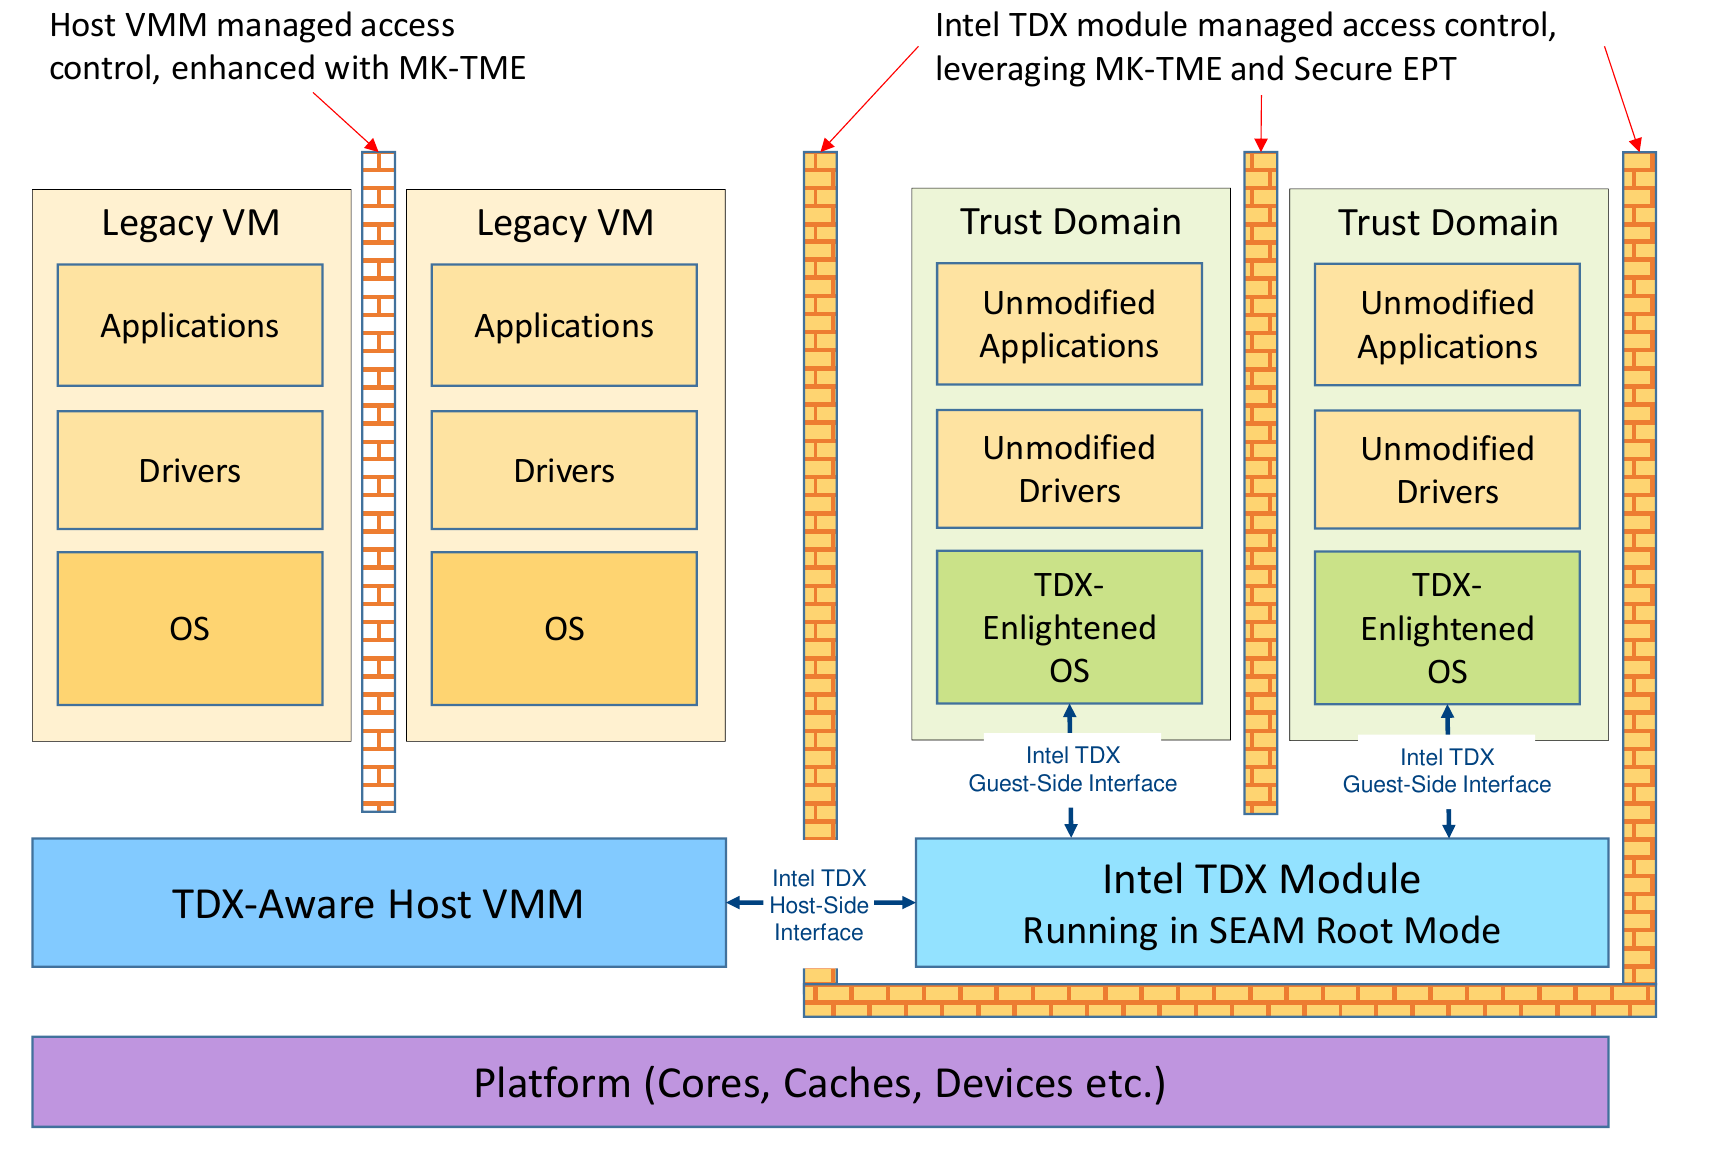
\includegraphics[width=\linewidth]{pictures/TDX_Arch.png}
  \caption{Intel TDX Components Overview \cite{Intel-TDX-Module-Specs}}
  \Description{Intel Trust Domain Extension Components Overview.}
  \label{fig:tdxcomponents}
\end{figure}

The first adversary is called a System Software Adversary which could be a compromised VMM, SMM, BIOS or other VMs.
This adversary basically covers every software based attack vector that that is not enabled through the TD itself or the firmware of the processor\cite[p. 8]{Intel-TDX-Whitepaper}.
A System Software Adversary is therefore able to read and write the complete system memory as well as access to the CPU state and the registers of the CPU.
Therefore the attacker has the ability to rewrite the page table to cause page table faults or remap/replay the memory pages of the TD.

The second adversary that is being considered is allowed to launch hardware attacks against Intel TDX.
This could be the Cloud Provider trying to extract information through attacks on the memory bus or other interfaces.
As this attacker has complete physical access to the hardware he is allowed to launch attacks like DRAM freeze or inject content into the DRAM through physical means\cite[p. 8]{Intel-TDX-Whitepaper}.

This means that the trusted components shown in \cref{fig:tdxcomponents} are the Platform (but only the CPU), and the Intel TDX Module as well as each Trust Domain in itself.
These components are also only part of the attestation as shown in \cite{CA-KVM}.
However it is also a good idea to extend the measurements to include the kernel and other subsequent components in the boot chain as this especially helps to protect in scenarios where the hoster of the VM is seen as untrusted but is providing a VM image to the user.
To allow the trusted firmware to measure the content of the kernel and subsequent components Trusted Platform Modules (TPM) can be used.
In order to efficiently scale virtualized TPMs (vTPM) can be used.
\sg{explain concept of vTPM}

\subsection{Previous Work}
\url{https://arxiv.org/pdf/2303.16463}

\subsection{Contributions}

This paper will explore the implementation of this technology in Intel TDX to see if vTPMs are a valid solution in order to establish a completely trusted chain.

\section{Background}

\subsection{Intel TDX}
% 1. Explain the general Architecture --> SEAM, TDX Module
Intel TDX short for Intel Trust Domain Extensions is an extension to the CPU architecture of Intels Xeon Scalable Processors since their 4th generation\cite{Intel-TDX-support}.
This technology implements as mentioned in the beginning a trusted execution environment where Virtual Machines are hardware isolated from the Virtual Machine Monitor (VMM), hypervisor and other software.
In order to ensure the complete isolation of the protected VMs (Trust Domain or TD) the CPU architecture has been extended through a software based component called the TDX Module as well as through extensions to x86 instruction set and other architectural changes.

\begin{figure}
  \centering
  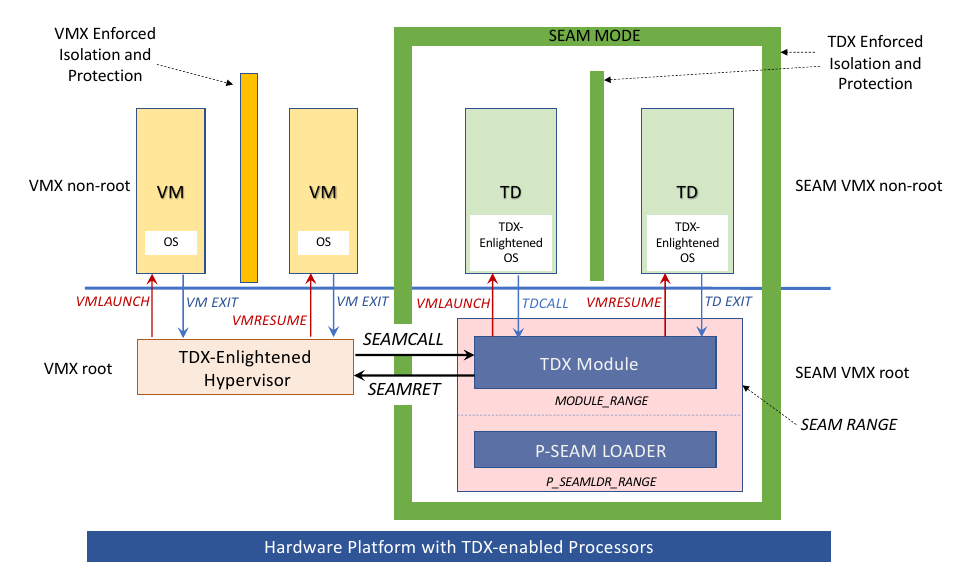
\includegraphics[width=\linewidth]{pictures/Intel_TDX_Architecture.png}
  \caption{Intel TDX Architecture via \cite{cheng2023intel}}
  \Description{Architecture of TDX and its SEAM mode}
  \label{fig:tdxarch}
\end{figure}

\subsection{TDX Module}
The core of the new system architecture is the new TDX Module with its loader as it can be seen in \cref{fig:tdxarch}.
The TDX Module itself is loaded as part of the bootchain through the P-SEAM Loader which is an Intel Authenticated Code Module (ACM).
These special code modules are loaded and verified by the CPU early in the boot process to ensure that they have not been manipulated.
Execution of these ACMs happens in on-chip memory which is called CRAM by Intel.
In addition to the TDX the hardware virtualization technique Intel VT was extended to cope with Trusted Domains.
In a classical scenario Intel VT operates in two modes the VMX root mode and the VMX non-root mode.
The VMX root mode allows privileged components like the hypervisor to access specific calls of the virtualization technology in order to control its guests.
The guest VMs typically run in the VMX non-root mode which introduces the Virtual Machine Control Structure (VMCS) which controls the CPU operations and can control how certain instruction behave. The VMCS allows to safe the state of VMs and therefore enables the pausing and switching between different VMs.
The non-root mode also seperates the address space between the hypervisor and the guest which prevents memory clashes\cite{VTx}.
For Intel TDX Intel VT got extended with a new mode called Secure Arbitration Mode (SEAM) which is responsible for the execution of TD.
The Intel TDX Module  and its loader are on the same privilege level as the hypervisor and are therefore executed in the new SEAM VMX root mode, protected VMs are executed in the SEAM VMX non-root.

As it can be seen in \cref{fig:tdxarch} the TDX Module has the same privilege level as the hypervisor and the communication with TDs to the hypervisor and reverse is routed through the TDX Module.
In its role as the major trust anchor for the TDs the TDX Module ensures through this communication flow that request that come from the hypervisor do not pose a thread to the TDs or that TD request do not harm the TD.
During the operation of VMs it is normal that the VMs are exiting in order to be resumed at a later stage or to request additional devices or information from the hypervisor.
To request device emulation or additional information from the hypervisor and context switch from the SEAM mode to the normal operation mode is required.
The TDX Module ensures in this scenario that the TD which just exited does not leak information to the untrusted hypervisor.

\subsubsection{Memory Encryption and Integrity}

In order to protect against a malicious hypervisor and other malicious VMs not only the communication between the hypervisor and the VM needs to be checked and secured but also the resources used by the TD.
Therefore the memory which is used by a TD is encrypted using the Intel Multi Key Total Memory Encryption (MKTME) technology.
During the creation of a TD a unique ephemeral encryption key is generated which is used to encrypt and decrypt the memory pages that belong to the TD.
As the encryption key is generated by the CPU it is not visible to the software and can not be exchanged\cite{Intel-MKTME}.
The protection of the memory is also extended through an integrity method as the encryption algorithm AES-XTS itself does not have any integrity measurements.
Memory integrity protection is achieved through two different methods.
The first method ensures that when a TD makes a request to retrieve content from its memory that the memory page that has been requested is indeed a private memory page.
This method is called Logical Integrity (LI) and only provides limited security\cite[p. 120]{Intel-TDX-Module-Specs}.
The second method Cryptographic Integrity (CI) provides an additional MAC.
This MAC is computed for each cache line together with the encryption tweak key and the TD owner bit with HMAC-SHA3-256 as the underlying algorithm\cite[p. 3]{Intel-TDX-Whitepaper}.
Afterwards the MAC is shortened to 28 bits and stored in the ECC region of the memory.
This provides the necessary isolation and protection against a malicious hypervisor.

\subsubsection{Remote Attestation}

Another important concept in the Intel TDX architecture is the possibility of remote attestation.
Attestation is a process where a server can prove to a challenger via a secure channel that certain configuration parameters are met and that the server is trustworthy.
In the context of confidential cloud computing this is an essential feature as the trusted resources are outside of the control of the user.
To achieve remote attestation the user first needs to establish a secure connection (SSH, TLS etc.) to a TD.
Afterwards a special CPU instruction can be invoked which creates a report for that specific TD.
The report includes information about the Trusted Computing Base (TCB) and other measurements about the TD like the virtual firmware which were measured during the building process of the TD.
The generated report is protected through the usage of a MAC which has been generated with a key that is only known to the CPU itself.
In a second step the report is passed to the quoting enclave (QE), which is already present since the introduction of Intel SGX.
A Quoting Enclave is able to verify that the report that has been sent to it was generated on the same platform through a secure manner and has not been manipulated.
Afterwards the Quoting Enclave will transfer the report into a Quote which can be verified off platform by a different entity.
The off platform verification can be achieved because the quote is through the private key of the quoting enclave which in turn is signed through the Provisioning Certification Enclave (PCE).
Signing the key of the QE needs to be done because in the Data Center Attestation Primitives (DCAP) model a vendor can specify its own QE.
However in order to ensure the hardware root of trust the QE needs to be signed through a Intel controlled and signed enclave which is the PCE.
The PCE is the only enclave allowed to retrieve a key for signing other enclaves which is derived from the hardware embedded keys\cite{Intel-QVL}.
Through this chain of signatures the challenger can contact an Intel service which has retained the hardware embedded key and ask it to verify that the signatures of the generated quote are correct.
Verifying the signature chains gives the challenger the security that an authentic Intel TDX enabled platform was used and therefore that the collected measurements are correct.
Now it is up to the challenger to interpret the measurements to conclude if the platform meets the expected security level or not.

The remote attestation however usually covers only the inital firmware of the VM and the platform information\cite{CA-KVM}.
Intel TDX is also able to cover additional information through the usage of 4 Runtime Measurement Registers (RTMR)\cite{CA-KVM}.
The RTMRs can be used to also cover the kernel as well as initrd and the whole userspace.
Covering the userspace and all applications makes the measurement unflexible and depending on the size of the installation may also have additional performance impacts\cite{CA-KVM}.
Therefore one approach is to measure only the platfomr and firmware and afterwards use firmware based attestation together with Trusted Platform Modules, more on that in \cref{chap:TPM} and \cref{chap:vTPMTDX}.

\begin{figure}
  \centering
  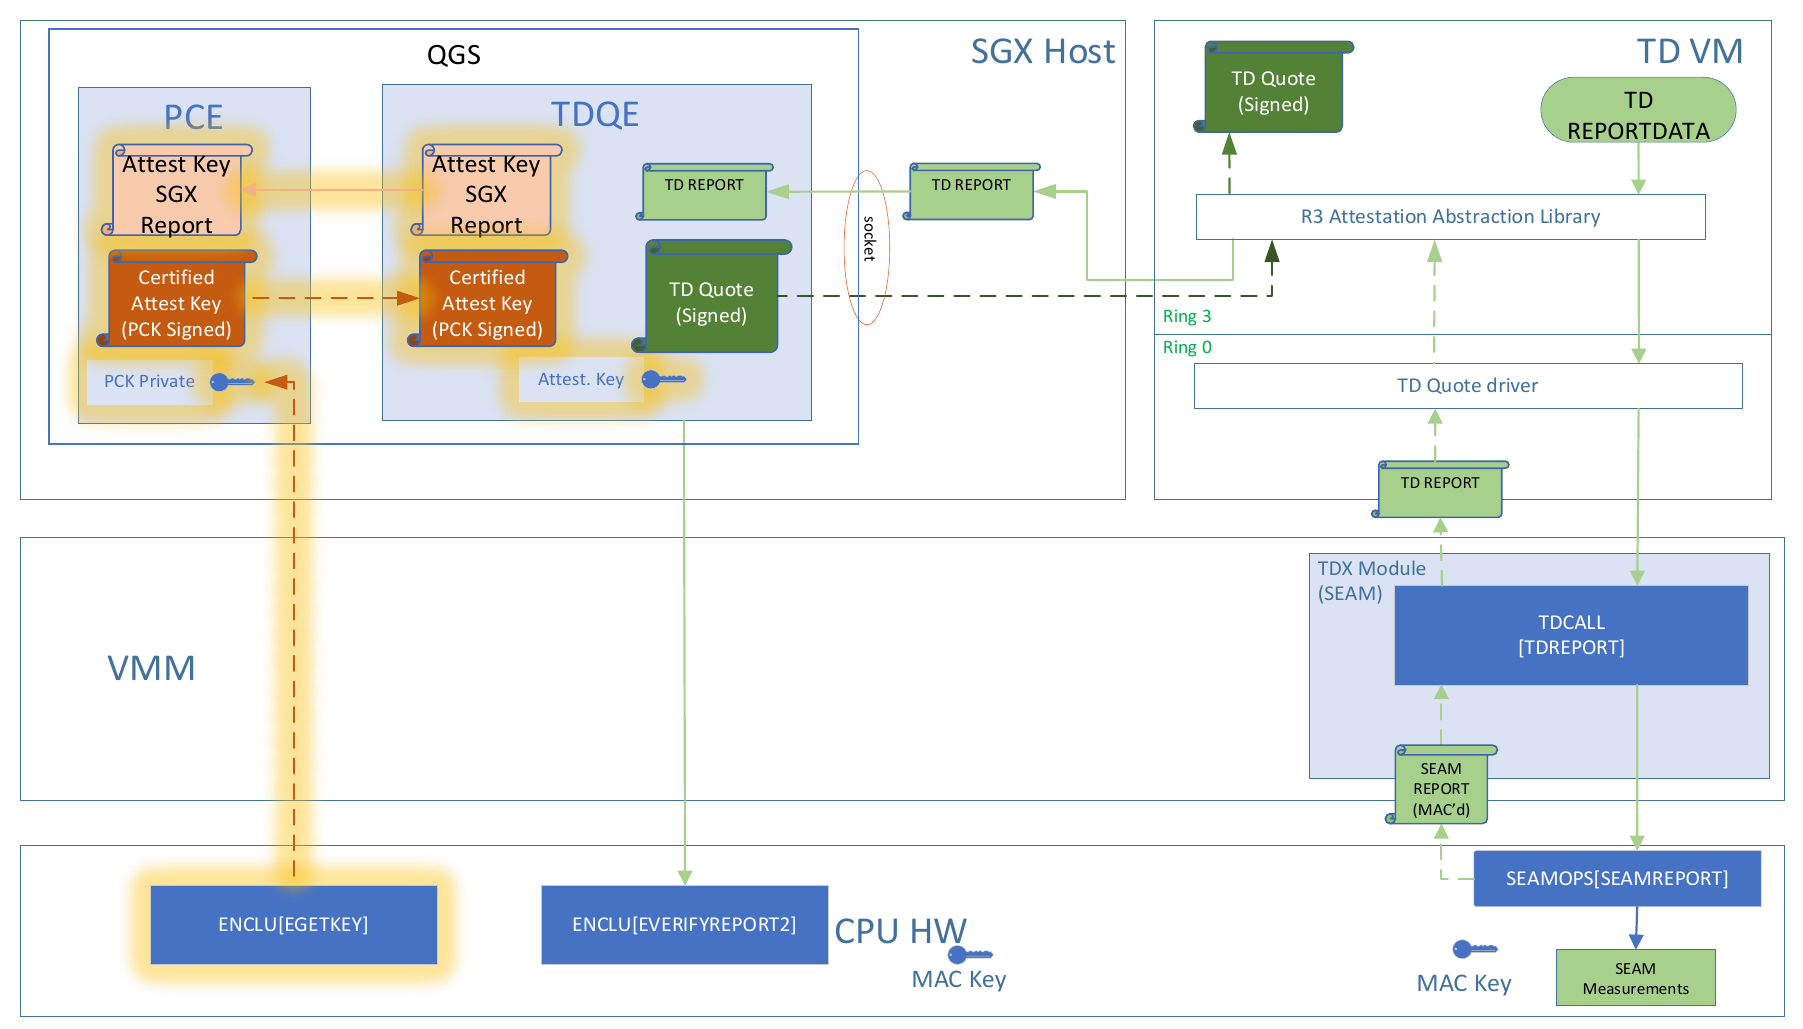
\includegraphics[width=\linewidth]{pictures/Enclaves.png}
  \caption{Intel TDX Attestation Architecture \cite{Intel-QVL}}
  \Description{Architecture of TDX Attestation and how the quotes and reports are getting generated.}
  \label{fig:tdxattest}
\end{figure}


\subsection{TPMs and vTPMs}
\label{chap:TPM}
% History of TPMS and vTPMS
% What are they?
% How do they work
% What is their main purpose
\sg{push to Background}
\sg{introduce and explain basic functions: crypto engine and storage, opt. secure channel to TPM, TPM identity/PKI; use cases: measured boot, secure boot, platform attesattion, give an example like disk encryption key provisioning}
A Trusted Platform Module short TPM is defined as a hardware root of trust which is recognised as more secure than a pure software implementation\cite[p.1]{TPM}.
The specifications of the TPM are developed by the Trusted Computing Group and are today widely in use by different technologies like Intel TXT\cite[p.15]{Intel-TXT} or Microsoft Bitlocker\cite{Bitlocker}.
As part of its special position the TPM provides security capabilities like random number generators, key generation and storage as well as different cryptographic algorithms.
All these functions are implemented in hardware and are resilient against tampering.
This ensures that secrets can be generated and stored safely.

However not all TPMs are bound by the hardware root of trust.
TPMs that are bound by the hardware root of trust are also often called discrete TPMs.
These TPMs provide the highest level of security and is hardened against sophisticated attacks and are mostly used in high risk environments.
Therefore a descrete chip is designed and built which undergoes several evaluations to check if it is resistent to hardware tampering attacks\cite{TPM-short}.

So called integrated TPMs are hardware implementations of TPMs that are integrated into another chip which provides functions that are not focused on security.
While still being a hardware implementation the TPM does not have the same level of tamper resistance\cite{TPM-short}.

Another class of TPMs are firmware TPMs.
A firmware TPM is implemented in the protected software (firmware) of the CPU without a dedicated TPM chip being required.
The firmware TPM typically resides within a TEE and is therefore separated from other programs that are being executed on the CPU.
Implementing a firmware TPM is much more cost efficient as dedicated hardware chips are no longer a requirement however the TPM now has a bigger attack surface through the TEE code and no longer being tamper resistant\cite{TPM-short}.

In the context of cloud computing TPMs that are fully implemented in software have been introduced.
These TPMs are under the control of the hypervisor which can make the TPMs available to the different Virtual Machines.
The hypervisor is able to create and destroy TPM instances as needed.
In the classical virtualization model the hypervisor is a trusted component and is responsible for the separation of the different Virtual Machines.
Therefore the virtualized TPMs (vTPM) can be seen as trusted.
However similar to the firmware TPMs the attack surface has increased and no hardware resistant tampering is possible\cite{perez2006vtpm}\cite{vTPM-google}.
\sg{explain how vTPMs realize the feature currently (note: insecure) and with help of TDs}



\section{vTPMs in Intel TDX}
\label{chap:vTPMTDX}

\subsection{Implementation in Intel TDX}
For the upcoming version of Intel TDX 1.5 a possibility was added to use vTPMs with Intel TDX.
However in contrast to the already known vTPMs that are in use today these vTPMs are not managed by the VMM as the VMM is an untrusted component in the Intel TDX security model.
Therefore a special implementation of vTPMs was developed which relies on the promised security guarantees from TDs.

In order to implement a vTPM within the Intel TDX architecture either a VM based approach can be used or a TDX module based approach could be used.
Implementing a vTPM within the TDX module is challenging as the TDX module itself is imposing a few limitation due to its major role in the software stack.
Introducing a vTPM functionality to the TDX Module would mean that the TCB itself is increasing due to the additional complexity introduced which is unwanted due to the major security role of the TDX Module\cite[p. 4]{Intel-vTPM}.
Other reasons why this approach is not favored is the dependency on Non-Volatile storage for a TPM and a long latency in order to generate keys\cite[p. 4]{Intel-vTPM}.

Therefore an TD-based solution has been implemented with two different designs where the vTPM is either in its own separate TD or in case of nested virtualization in the level 1 VM which hosts the VMM for the nested virtualization.
As the vTPM shall work together with the existing TDX 1.0 architecture where nested virtualization is not supported the focus will be on the first solution where the vTPM is hosted in its own TD\cite[p. 5]{Intel-vTPM}.
In addition the vTPM TD shall follow the TPM 2.0 specifications and shall not modify the TPM Software Stack as this ensures the compatability with existing guidelines and implementations\cite[p. 5]{Intel-vTPM}.
However the vTPM TD cannot fulfil the requirement of the persistent Non-Volatile storage due to its virtualization nature e.g. the hypervisor is able to delete the VM.

As the implementation relies on a separate TD which hosts the vTPM the VVM is responsible for launching the TD and afterwards creating the vTPM instance.
After the vTPM instance has been created it initializes itself and therefore produces the Endorsement Key (EK) which is a unique asymmetric key for each TPM.
The whole process is shown in \cref{fig:vtpmlaunch}.

\begin{figure}
  \centering
  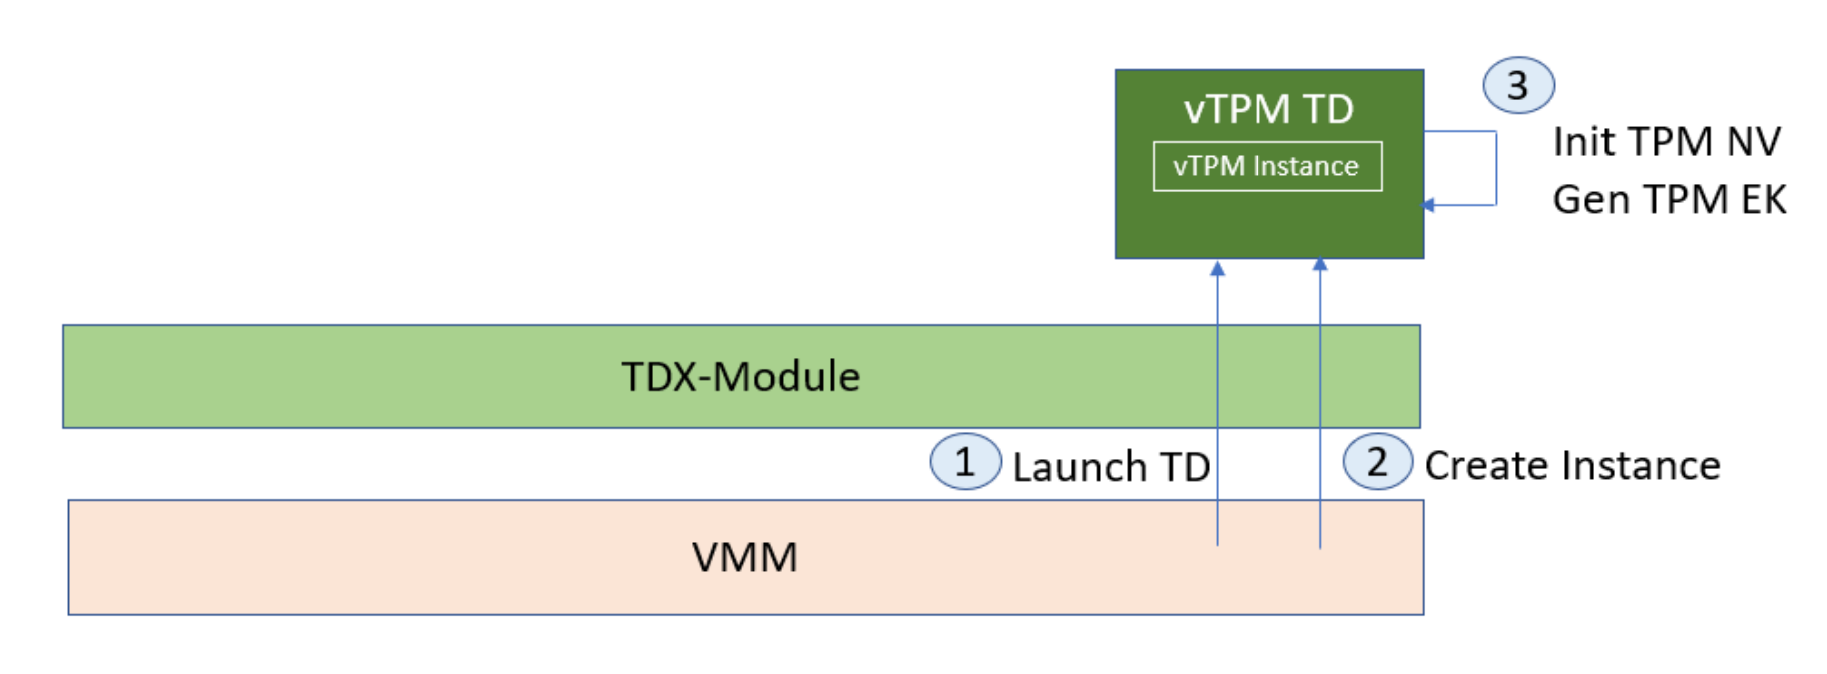
\includegraphics[width=\linewidth]{pictures/vTPM_launch.png}
  \caption{Intel TDX vTPM launch flow \cite{Intel-vTPM}}
  \Description{The launch flow of the vTPM TD illustrated with the TDX-Module and VMM.}
  \label{fig:vtpmlaunch}
\end{figure}

If a user TD with TPM support is launched the user TD establish a secure connection to the vTPM TD and attests the vTPM TD, while the vTPM TD attests the user TD.
As both parties can be sure that they are communicating over a secure channel with another TD the vTPM stores the TDREPORT within its PCR-Banks.
The user TD on the other hand includes the session info in the RTMR[3] in order to have the evidence that a vTPM is connected and can be used.
This simplified flow can be seen in \cref{fig:vtpmlaunchusertd}.

\begin{figure}
  \centering
  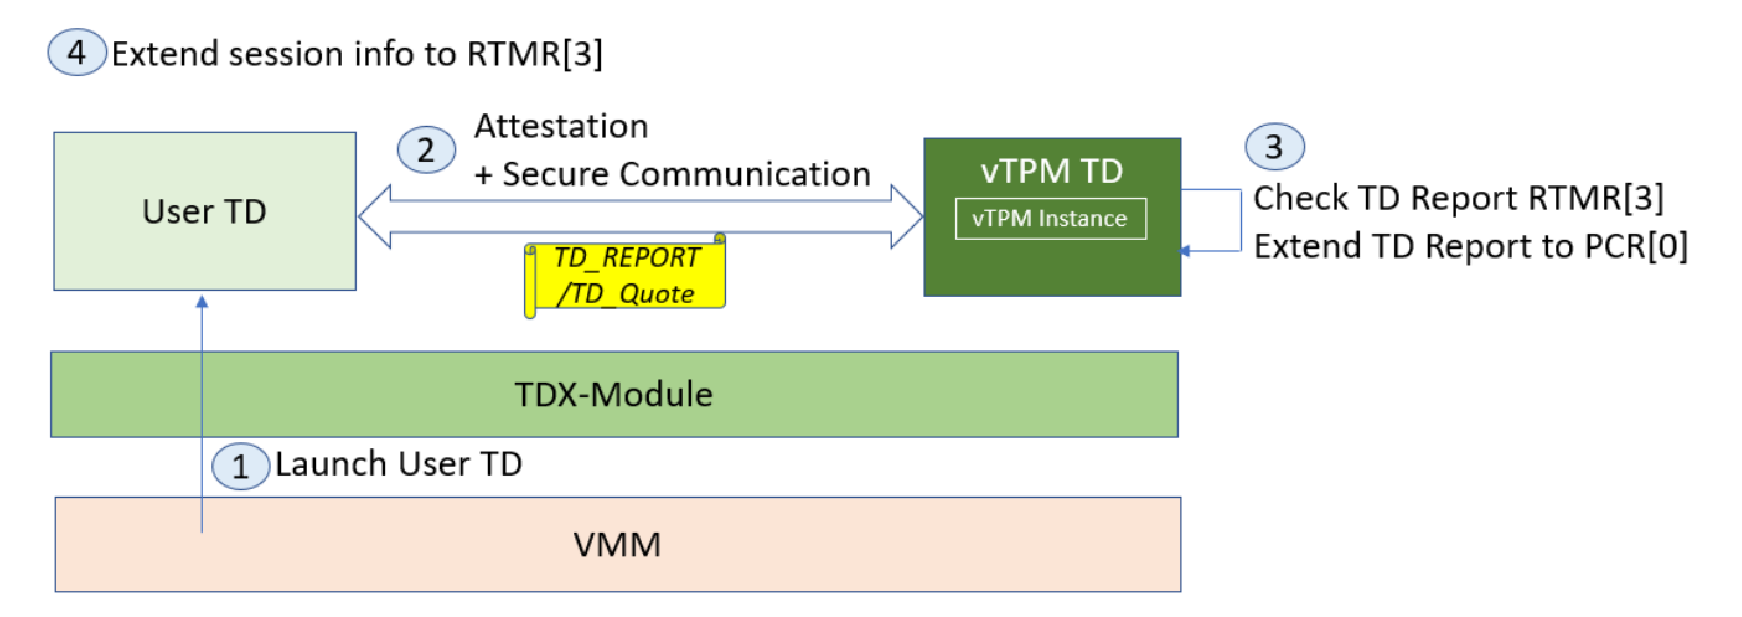
\includegraphics[width=\linewidth]{pictures/vTPM_TD_launch.png}
  \caption{Intel TDX vTPM User TD launch flow \cite{Intel-vTPM}}
  \Description{The launch flow of the User TD together with a vTPM illustrated with the TDX-Module and VMM.}
  \label{fig:vtpmlaunchusertd}
\end{figure}

 The communication flow between the user TD and the vTPM TD for the exchange of commands and the response is not as simple as shown in \cref{fig:vtpmlaunchusertd} as the user TD and vTPM TD need to communicate through the VMM with each other which involves many calls like shown in \cref{fig:vtpmcommunication}.

The vTPM TD and user TD are both extended with a command-response-buffer (CRG) in order to communicate with each other.
\sg{how is the initial shared key established?}
The buffer therefore resides in the shared memory regions and is accessible by the VMM and due to that the TPM command and its response which are exchanged through this buffer are enccrypted with an Authenticated Encryption with Associated Data (AEAD) algorithm in order to protect it against a malicious VMM.
The encryption uses two separate keys the AEAD requester key and the AEAD responder key.
Both keys are known to the user TD as well as the vTPM TD.

The communication flow contains the following steps:
\begin{enumerate}
    \item The user TD selects the necessary TPM command and supplies the necessary information and afterwards encrypts the message with the AEAD requester key which is subsequently copied into the CRB for the TPM.
    \item The user TD can use the Guest-Host-Communication-Interface (GHCI) TDG.VP.VMCALL<\textbf{Service.vTPM}> call to notify the VMM that an action for the specified service is pending.
    \item The VMM copies the encrypted TPM command from the shared memory of the user TD into the shared memory of the vTPM TD.
    \item The VMM notifies the vTPM TD that the vTPM has been written to its CRB and can now be processed.
    \item After the vTPM TD has received the notification it copies the command from the CRB into its private memory and decrypts the TPM command with the AEAD requester key which enables the vTPM to process the command.
    \item After successfully processing the TPM command the response is getting encrypted with the AEAD responder key and written back to the CRB.
    \item The vTPM can now also use the GHCI with \\TDG.VP.VMCALL<\textbf{Service.vTPM}> to notify the VMM.
    \item The VMM copies the encrypted TPM command from the CRB of the vTPM TD to the CRB of the TD.
    \item The VMM notifies the user TD that the response has been written to the CRB and can now be processed.
    \item After the user TD has received the notification it copies the response from the CRB into its private memory and decrypts it using the AEAD responder key. 
\end{enumerate}
% Docs state last point wrong they user requester key while it should be responder key

\begin{figure}
  \centering
  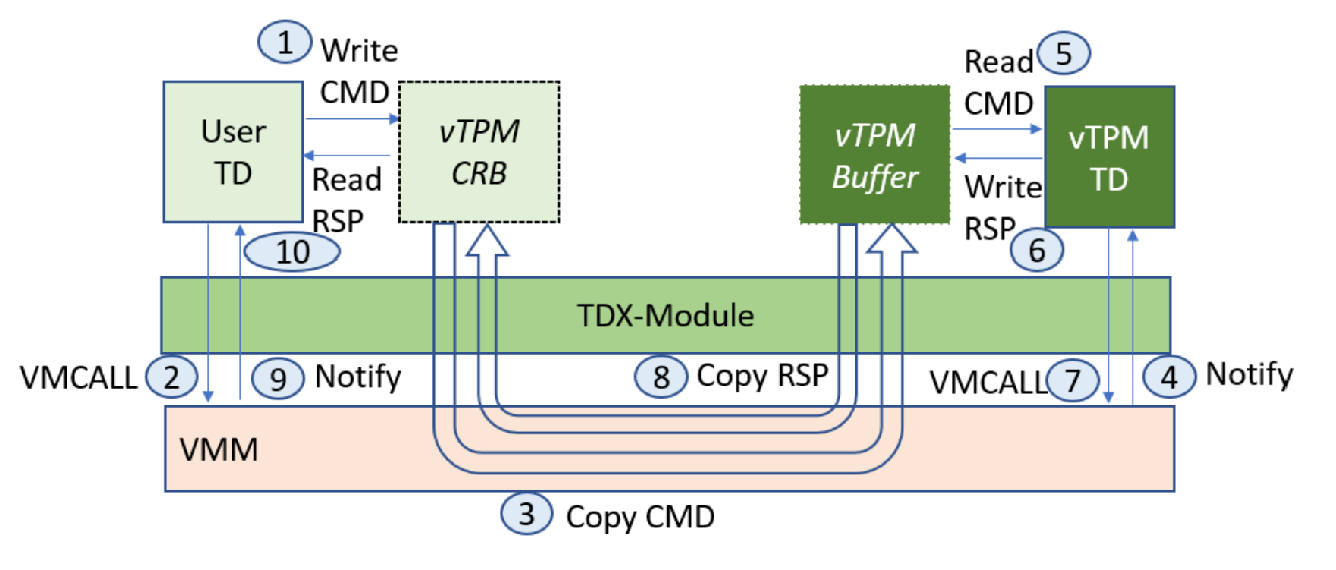
\includegraphics[width=\linewidth]{pictures/vTPM_communication.png}
  \caption{Intel TDX vTPM User TD runtime communication flow \cite{Intel-vTPM}}
  \Description{The runtime communication flow of the User TD together with a vTPM illustrated with the TDX-Module and VMM.}
  \label{fig:vtpmcommunication}
\end{figure}

\subsubsection{Trust Relationship}
As the client of the vTPM the user TD generally places a lot of trust in the vTPM while the vTPM as the root of trust does not trust the user TD.
The user TD itself will only trust the vTPM TD after the virtual firmware of the TD has verified that the report or quote which has been sent from the vTPM TD is valid.
To communicate with the vTPM TD a secure session via SPDM or TLS is established and after successful verification of the Quote or TDREPORT extended to the user TD and stored in RTMR[3].
If the connection however should fail a random value is written to RTMR[3] in order to indicate that the connection failed.
Due to the limitations of the user TD it can generally not verify if the vTPM TD is acting malicious however once the verifier request a complete verification process which includes the measurements of the vTPM this can be detected through the Endorsement Key of the vTPM.

In contrast to the user TD a vTPM TD only trusts the TDX Module.
Therefore the vTPM records all TDREPORTs that have been received over the secure session in order to prevent the TDVF from forging any measurements.
As the TDREPORT is generated through the TDX Module it can be trusted after a successful verification.
In order to protect fully against forged measurements from the TDVF the vTPM TD needs to ensure that the TDVF itself is not malicious.
A detection is possible because the TDX Module itself measures the TDVF and includes it in the Measurement of Trust Domain (MRTD which subsequently can be checked by the verifier.
An additional protection against forged measurements from the guest OS is that the vTPM verifies that the secure session is initiated by the TDVF.
This is achieved through checking the RTMR[3] in the TDREPORT to be zero and rejecting the session if the RTMR[3] is non zero.

\subsubsection{Usage in Attestation}
With the Introduction of the vTPM a TD can choose if it wants to use the standard RTMR based remote attestation flow or if it wants to use the remote attestation flow of the vTPM.
Choosing the vTPM based attestation allows the verifier to verify additional properties of the user TD through the additional PCR banks of the vTPM which can contain measurements of the installed applications or anything else, while the RTMR based remote attestation flow is limited to the measurement of the hardware and firmware.
As the TDREPORT of the user TD is also stored in the PCR[0] bank which is transmitted to the verifier in the vTPM based attestation a verification of the user TD is still possible with this new attestation flow.
However a TD can not support both attestation flows as this could cause a mismatch in the attestation phase because a verifier may only be aware of the RTMR based attestation.
If the verifier now tries to attest a vTPM flow this would not work even if the verifier retrieves the TDREPORT or TDQUOTE for the user TD the verification would not work as the vTPM based flow poisons the RTMR register 0 through 2.

A vTPM can also be used for measurements made by the Linux Integrity Measurement Architecture (IMA) which enables support for runtime measurements\cite{Intel-IMA}.
The IMA allows to detect if files which are part of the measurement have been altered either by accident or through another malicious program.

\subsection{Security Considerations}
As the vTPM TD is being launched through the VMM which itself is an untrusted component it needs to be ensured that the provided vTPM Instance has not been manipulated.
In a guide provided by Intel the vTPM is provided to the VMM as a binary and launched through the libvirt loader parameter which usually indicates that a firmware blob is used\cite[p. 84]{Intel-linux-tdx}\cite{libvirt}.
As it is recommended to use the TDX Virtual Firmware Design Guide for the vTPM TD binary it can be safely assumed that the vTPM TD is indeed a part of the firmware\cite[p. 20]{Intel-vTPM}.
This is in line with the information that the vTPM TD is a lightweight bare-metal TD which is part of the TCB and therefore should be as minimal as possible\cite[p. 18]{Intel-vTPM}.
That the vTPM binary blob is part of the firmware is a crucial point as otherwise the VMM could easily swap the binary blob out and the verifier could never verify if the binary blob has been exchanged.

In order to additionally reduce the risk of errors within the vTPM TD proven cryptographic implementations should be used as well as proven implementations of the TPM functionality.
For low level hardware programming typically C or C++ is the choice however Intel recommends to use type safe languages to eliminate memory safety issues\cite[p. 20]{Intel-vTPM}.
The reference implementation by Intel is therefore written in Rust\cite[p. 20]{Intel-vTPM}.

Due to the nature of vTPMs the Endorsement Key of a vTPM is generated upon creation of the vTPM and destroyed after the tear down of the instance or VM.
On hardware based TPMs the Endorsement Public Key is usually included in the Endorsement Key Certificate which is signed by the manufacturer and included in the TPM.
Including the Endorsement Key Certificate in the TPM allows the verifier to attribute the TPM to a specific manufacturer.
By default a vTPM can not provide this traceability and accountability.
However it is possible to setup a Certificate Authority (CA) which will receive a TD Quote including the Endorsement Public Key.
After verifying the quote and checking that the firmware which the vTPM is a part of has not been manipulated the CA can sign the Endorsement Public Key and issue a certificate that this key is a genuine key which was produced through an approved vTPM.
Sending the certificate back to the vTPM allows the vTPM to prove that is a genuine vTPM which has been setup and verified by the Certificate Authority.

\subsection{Similiar approaches}
CoCoTPM short for Confidential Computing TPM is a proposed vendor neutral design for the usage of TPMs in Confidential Computing VMs.
The concept generally involves a seperate CoCoTPM VM and a Kernel and UEFI Level CoCoTPM driver to allow communication between the CC-VM and the CoCoTPM VM \cite[3]{10.1145/3564625.3564648}.
As the proposed concept is generally vendor neutral no specifications are made available on how the VMs should communicate the encrypted TPM commands to the Hypervisor or the other VM.
However the basic concept of spawning an additional VM which implements the TPM functionality and provides the TPM functionality to another VM via a secure channel and encrypted TPM commands is the same as the implementation for Intel TDX.

A non vendor neutral design has been proposed in \cite{10.1145/3627106.3627112} and is focused on AMD-SEV.
This design uses the Secure VM Service Module which is a guest communication interface that allows to offload workloads to another VM which runs with more privileges (Virtual Machine Privilege Level is a new concept introduced by AMD which blocks certain instructions for guests with lower privileges).
This allows to securely pass the execution of a certain command or feature to a VM with more privileges and eliminating the need for extending the TCB with additional protocl implementations like SPDM or TLS.

\section{Conclusion}
Implementing secure vTPMs in Intel TDX through the usage of a separate VM is a feasible approach and allows to extend the measurement from the firmware level to the complete software stack.
While the current architecture of Intel TDX has the need for increasing the TCB through the usage of standard protocols like SPDM or TLS instead of being able to use CPU embedded features to securely exchange information between VMs this is only a limited risk when well audited codebases are used that do not posess more capabilities than required.
In addition the support for vTPMs allows to use the standardized attestation interface of vTPMs instead of the vendor specific communication interfaces.
However in order to completely verify the attestation provided by the vTPM vendor specific checks are still required.

\bibliographystyle{ACM-Reference-Format}
\bibliography{main}


\end{document}